\chapter{Lokaler Planer: Dynamic Window Appraoch}
Nachdem die Berechnung eines Pfades zwischen Ausgangs- und Zielposition mittels $A*$ gelöst wurde, muss als nächstes eine Folge von Steuerkommandos ermittelt werden, um den geplanten Pfad abzufahren. Den Ausgangspunkt stellt die Dynamik des roboters dar: Die Position des Roboters wird in dem Zustandsvektor 
\begin{equation}
\mVec{x}(t) = \begin{pmatrix}
x \\ y \\  \theta
\end{pmatrix}
\end{equation}
erfasst, wobei die ersten beiden Größen die Position und der Winkel $\theta$ die Blickrichtung des Roboters beschreiben. Nach wie vor gilt die Annahme, dass der Roboter in einer planen Umgebung manövriert. Die Positionsänderung wird mithilfe einer Translationsgeschwindigkeit $v$ und einer Rotationsgeschwindigkeit $\omega$ erfasst, die wiederum in dem Vektor
\begin{equation}
\mVec{u} = \begin{pmatrix}
v \\ \omega
\end{pmatrix}
\end{equation}
zusammengefasst werden. Bei den Turtlebots werden die Motoren drehzahlgeregelt, weshalb der Geschwindigkeitsvektor $\mVec{u}$ die Stellgröße zur Ansteuerung des Roboters darstellt. wird die Annahme getroffen, dass die an einem Zeitpunkt $n\cdot T\idx{a}$ eingestellt Geschwindigkeit für die folgende Abtastperiode konstant ist, kann die Positionsänderung in X- und Y-Richtung mittels der folgenden Gleichungen berechnet werden:
\begin{equation}
x\idx{n+1} = x\idx{n} + \Delta x(n)
\end{equation}
\begin{equation}
y\idx{n+1} = y\idx{n} + \Delta y(n)
\end{equation}
\begin{equation}
\Delta x(n) = \left\{ \begin{array}{ll}
\frac{v\idx{n}}{\omega\idx{n}}\cdot \left( \mSin{\theta\idx{n}}-\mSin{\theta\idx{n}+\omega\idx{n}\cdot T\idx{a}}\right) & \hspace{1cm} \forall \omega\idx{n} \neq 0 \\
v\idx{n}\cdot \mCos{\theta\idx{n}}\cdot T\idx{a} & \hspace{1cm} \forall \omega\idx{n} = 0 \end{array}\right.
\end{equation}
\begin{equation}
\Delta y(n) = \left\{ \begin{array}{ll}
-\frac{v\idx{n}}{\omega\idx{n}}\cdot \left(\mCos{\theta\idx{n}}-\mCos{\theta\idx{n}+\omega\idx{n}\cdot T\idx{a}}\right) & \hspace{1cm} \forall \omega\idx{n} \neq 0 \\
v\idx{n}\cdot \mSin{\theta\idx{n}}\cdot T\idx{a} & \forall \omega\idx{n} = 0
\end{array}\right.
\end{equation}
Aus den zeitweise konstanten Geschwindigkeiten resultiert eine Kreisbahn mit dem Radius $v\idx{n} / \omega\idx{n}$ im Falle, dass $\omega\idx{n} \neq 0$ gilt. Im Extremfall mit $\omega\idx{n} = 0$ bewegt der Roboter sich rein translativ entlang einer Geraden. Somit wird der Raum der möglichen Trajektorien auf Kreisbahnen reduziert, wodurch die Komplexität des folgenden Suchproblems drastisch reduziert wird.

Unter den obigen Annahmen soll nun ein Geschwindigkeitsvektor $\mVec{u}$ gewählt werdne, um den Roboter in Richtung eines gegebenen Zielpunktes zu fahren, der in der nähren Umgebung liegt. Im ersten Schritt wird der Versuch unternommen, den Suchraum der möglichen Geschwindigkeiten durch Nebenbedingungen weiter einzugrenzen. Sowohl für die Translations- als auch die Rotationsgeschwindigkeit bestehen Maxima, die nicht überschritten werden dürfen, woraus die Menge
\begin{equation}
V\idx{s} = \left\{ (v,\omega) \mCond v < v\idx{max} \land \omega < \omega\idx{max}\right\}
\end{equation}
resultiert. Neben den Geschwindigkeiten sind auch die Beschleunigungen beschränkt, weshalb die Menge der erreichbaren Geschwindigkeiten durch die aktuellen Geschwindigkeiten  $v\idx{a}$ und $\omega\idx{a}$, und die maximalen Beschleunigungen eingeschränkt werden.
\begin{equation}
V\idx{a} = \left\{ (v,\omega) \mCond v \in \left[v\idx{a}-\dot{v}\idx{max}\cdot T\idx{a}, v\idx{a}+\dot{v}\idx{a}\cdot T\idx{a}\right] \land \omega \in \left[\omega\idx{a}-\dot{\omega}\idx{max}\cdot T\idx{a}, \omega\idx{a}+\dot{\omega}\idx{max}\cdot T\idx{a}\right] \right\}\,.
\end{equation}
Als dritte Begrenzung des Suchraums werden Hindernisse in der Umgebung herangezogen. Jedem Geschwindigkeitsparr $(v,\omega)$ kann eine Kreisbahn zugeordnet werden, wobei die Funktion $\text{dist}(v,\omega)$ die Distanz des nächsten Hindernisses am Ende der Abtastperiode auf der zugehörigen Kreisbahn wiedergibt. Wenn nun eine maximale Verzögerung von $\dot{v}\idx{max}$ und $\dot{\omega}\idx{max}$ erreicht werden kann, folgt für die maximal erlaubte Geschwindigkeit, um vor dem Hindernis bremsen zu können:
\begin{equation}
V\idx{d} = \left\{ (v,\omega) \mCond v \leq \sqrt{2\cdot \text{dist}(v,\omega)\cdot \dot{v}\idx{max}} \land \omega \leq \sqrt{2\cdot\text{dist}(v,\omega)\cdot \dot{\omega}\idx{max}} \right\}\,.
\end{equation}
Der Raum der zulässigen Geschwindigkeiten ergibt sich aus dem Schnitt der drei Mengen
\begin{equation}
V = V\idx{s} \cap V\idx{a} \cap V\idx{d}\,.
\end{equation}
Nun gilt es eine Geschwindigkeit aus dem Suchraum $V$ auszuwählen, wofür wiederum ein Gütekriterium definiert wird, dessen Optimum erzielt werden muss. Bei der Auswahl der Zielfunktion werden drei Aspekte berücksichtigt: Der Roboter soll sich möglichst weit in Richtung des Zielpunktes bewegen, die Blickrichtung des Roboters soll am Ende der folgenden Abtastperiode auf den Zielpunkt gerichtet sein, und die Distanz zwischen dem Roboter und Hindernissen soll möglichst groß gehalten werden. Diese drei Teilziele werden jeweils durch eine separate Funktion beschrieben, deren Summe bei der Suche maximiert werden soll. Die Richtungsabweichung wird durch die Funktion
\begin{equation}
\text{heading}(v, \omega) = \pi - \varphi \hspace{1.5cm} \varphi = \sphericalangle 
\end{equation}
erfasst, wobei $\varphi$ den Winkel zwischen Blickrichtung und Zielpunkt beschreibt. Die Gewichtung der Geschwindigkeit erfolgt mittels einer simplen Gerade der Form
\begin{equation}
\text{velocity}(v, \omega) = a\cdot v\,.
\end{equation}
Um den Abstand von Hindernissen zu bewerten, wird wieder die bekannte Funktion $\text{dist}(v,\omega)$ verwendet, wobei zu beachten ist, dass im Falle einer Kurve ohne Hindernisse eine recht große Konstante zurückgeliefert wird. Zusammengeführt ergeben die einzelnen Teile die Zielfunktion
\begin{equation}
G(v, \omega) = \alpha\cdot \text{heading}(v,\omega)+ \beta\cdot \text{velocity}(v,\omega)+\gamma\cdot \text{dist}(v,\omega)\,,
\end{equation}
wobei die Faktoren $\alpha$, $\beta$ und $\gamma$ zur Normierung der Teilzielfunktionen verwendet werden. Dadurch wird sichergestellt, dass keine der drei Funktionen das Ergebnis der Optimierung überproportional beeinflusst.

\section{Anwendungsbeispiel}
Um die Funktionsprinzipien des lokalen Planers besser nachvollziehen zu können, wird an dieser Stelle schrittweise eine Implementierung erarbeitet, die anschließend in der Simulation verifiziert wird. Im ersten Schritt werden die Bedingungen für die zulässigen Geschwindigkeiten konstruiert, wofür Angaben für die maximalen Geschwindigkeiten benötigt werden. Diese werden im Datenblatt des TurtleBot \cite{TurtlebotDS} mit
\begin{equation}
v\idx{max} = 0.65 \hspace{2.5cm} \omega\idx{max} = \pi
\end{equation}
spezifiziert. Über die maximalen Verzögerung der Aktoren sagt das Datenblatt nichts aus, weshalb an dieser Stelle die Annahmen von 
\begin{equation}
\dot{v}\idx{max} = 0.65 \hspace{2.5cm} \dot{\omega}\idx{max} =  \pi 
\end{equation}
getroffen wird. Für die spätere Anwendung können die maximalen Beschleunigungen experimentell ermittelt werden und auch in der Simulation adaptiert werden. Die aktuellen Geschwindigkeiten $v\idx{a}$ und $\omega\idx{a}$ können den Odometriedaten entnommen werden, welche über die ROS-Topic \lstinline{\odom}{} veröffentlicht werden. 

Als letzte Einschränkung ist der Abstand zwischen nächstem Hindernis und dem Turtlebot zu beachten, der mithilfe der Funktion $\text{dist}(v,\omega)$ berechnet wird. Die Implementierung der Distanzfunktion macht sich wieder den Umstand zu nutzen, dass die Menge der möglichen Trajektorien begrenzt ist: Der Roboter bewegt sich auf einer Kreisbahn mit dem Radius $r=\frac{v}{\omega}$, deren Mittelpunkt $M$ simultan als Ursprung des Koordinatensystems verwendet wird. 
\begin{figure}[!ht]
\centering
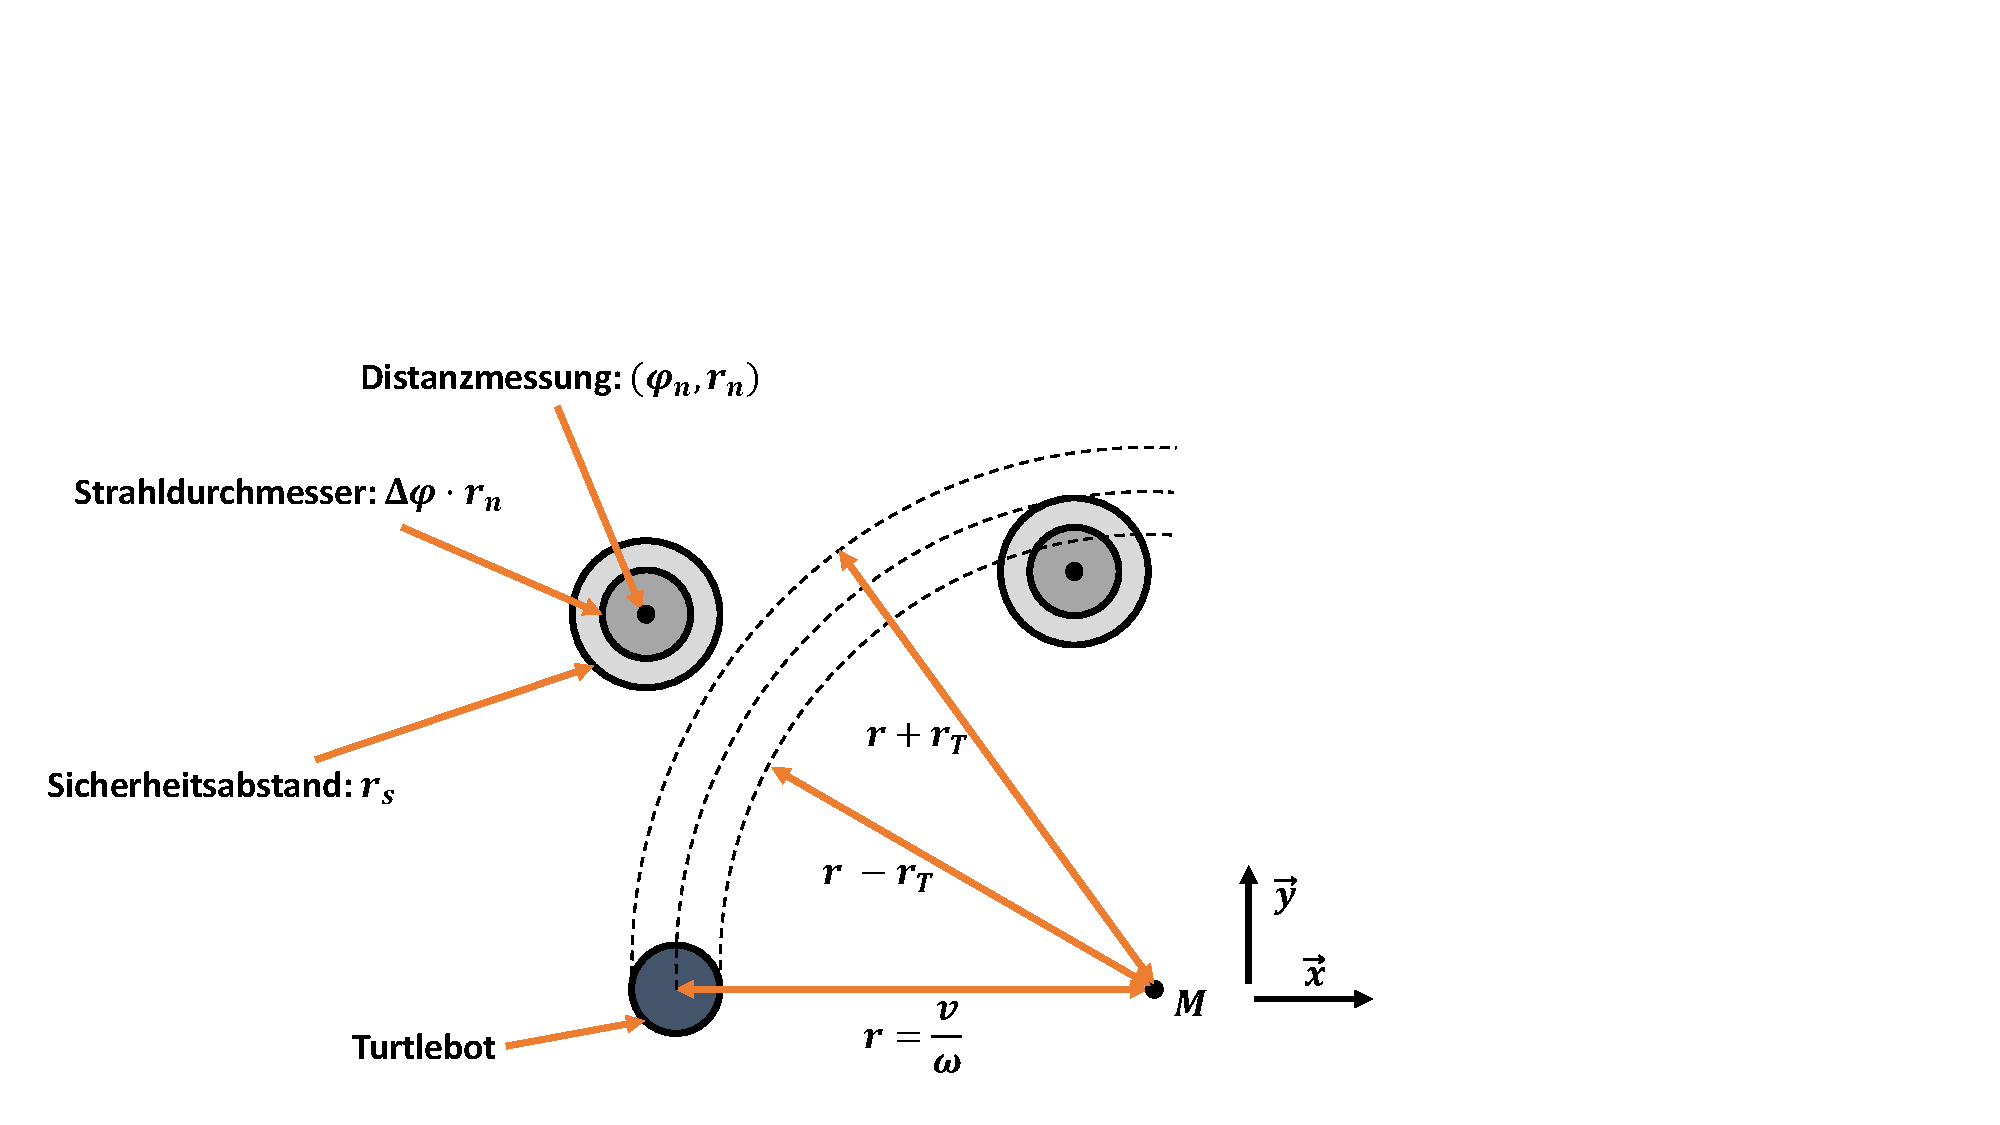
\includegraphics[width=0.7\linewidth, trim={0cm 0cm 10cm 6cm}, clip]{img/Distanz_img1}
\caption{Darstellung der Trajektorie und Hindernissen}
\end{figure}

Somit folgt für die Position des TurtleBot
\begin{equation}
\mVec{p}\idx{R} = \left\{\begin{array}{rl}
-\begin{pmatrix} r \\ 0 \end{pmatrix} & \hspace{1cm} \forall \omega < 0 \\
\begin{pmatrix} r \\ 0 \end{pmatrix} & \hspace{1cm} \forall \omega > 0 
\end{array}\right.\,,
\end{equation}
wobei der Fall $\omega = 0$ separat betrachtet werden muss. Da es sich bei dem Roboter um keinen Punkt sondern eine Kreisscheibe mit dem Radius $r\idx{R}$ handelt, wird ein Schlauch mit Innenradius $r\idx{I} = r - r\idx{R}$ und Außenradius $r\idx{A} = r + r\idx{R}$ überfahren. Diese Fläche kann in Polarkoordinaten als die Punktmenge
\begin{equation}
K\idx{R} = \left\{ (\phi, s) \mCond s \in \left[r\idx{I},r\idx{A}\right] \land \phi \in \left[0, 2\cdot \pi\right]\right\} 
\end{equation}
dargestellt werden.
Der Laserscanner liefert einen Messvektor $\mVec{z}$, dessen Element jeweils ein Paar $(\varphi\idx{n}, r\idx{n})$ sind, das sowohl den Winkel zwischen Messstrahl und Blickrichtung als auch die darauf gemessene Entfernung $r\idx{n}$ beschreibt. Folglich stellt das Paar die Position eines Messpunktes relativ zu dem TurtleBot dar, wobei die Darstellung in Form von Polarkoordinaten vorliegt. Liegt der Messpunkt zwischen den Kreisbahnen $r+r\idx{T}$ und $r-r\idx{T}$ blockiert er die Bahn des Roboters. Des Weiteren muss beachtet werden, dass eine finite Anzahlen von Messstrahlen vorliegt, weshalb jeder Messpunkt einen Messkegel mit Öffnungswinkel $2\cdot \Delta\varphi$ repräsentiert. Insofern ergibt es Sinn zu prüfen, ob der Kreis mit Mittelpunk $(\varphi\idx{n},r\idx{n})$ und Radius $\Delta\varphi\cdot r\idx{n}$ die Bahn des Roboters schneidet. Als zusätzliche Absicherung kann der Kreis um den Messpunkt um einen Sicherheitsabstand $r\idx{s}$ erweitert werden. Eine mathematische Formulierung resultiert, indem die Position des Messpunktes $\mVec{p}\idx{n}$ zunächst in dem Koordinatensystem dargestellt wird:
\begin{equation}
\mVec{p}\idx{n} = \mVec{p}\idx{R} + \begin{pmatrix} \mSin{\varphi\idx{n}} \cdot r\idx{n} \\ \mCos{\varphi\idx{n}}\cdot r\idx{n}\end{pmatrix}\,.
\end{equation}
Die im Kreis enthaltene Menge ergibt sich aus allen Punkten, deren Abstand zu dem Messpunkt kleiner als der Radius ist:
\begin{equation}
K\idx{M} = \left\{ \mVec{p} \mCond \mNorm{\mVec{p}-\mVec{p}\idx{n}} \leq \Delta\varphi\cdot r\idx{n} + r\idx{s}\right\}\,.
\end{equation}
Somit kann formal geprüft werden, ob das in einer Messung $(\varphi\idx{n},r\idx{n})$ identifizierte Hindernis auf einer durch das Geschwindigkeitspaar $(v,\omega)$ definierten Kreisbahn liegt. Ergibt der Schnitt der Mengen
\begin{equation}
K\idx{R} \cap K\idx{M}
\end{equation}
die leere Menge $\emptyset$, so wird die Trajektorie nicht von dem Hindernis blockiert. Allerdings stellt die Berechnung der Schnittmenge kein elegantes Verfahren dar, um die Position des Hindernisses zu prüfen. An dieser Stelle bietet es sich an, den Abstand $d$ eines Messpunktes $\mVec{p}\idx{n}$ zu dem Ursprung $M$ zu berechnen;
\begin{equation}
d = \mNorm{\mVec{p}\idx{n}}\,.
\end{equation}
Alle Punkte des Messkreises $K\idx{M}$ liegen zwischen dem maximalen Abstand
\begin{equation}
d\idx{max} = d + \Delta\varphi\cdot r\idx{n} + r\idx{s}
\end{equation}
und dem minimalen Abstand
\begin{equation}
d\idx{min} = d - \Delta\varphi\cdot r\idx{n} - r\idx{s}\,,
\end{equation}
wodurch sich die Prüfung auf eine simple Fallunterscheidung reduziert. Liegt einer der Abstände $d\idx{max}$ und $d\idx{min}$ zwischen den Radien $r\idx{A}$ und $r\idx{I}$, so blockiert das Hindernis die Kreisbahn. Das selbe Resultat ergibt sich in dem Fall, dass sowohl $d\idx{max} > r\idx{A}$ als auch $d\idx{min} < r\idx{I}$ gilt. Liegt ein Hindernis auf der Bahnkurve, so entspricht dessen Winkelposition $\gamma$ der Polarkoordinate des Messpunktes
\begin{equation}
\gamma = \sphericalangle \mVec{p}\idx{n}\,,
\end{equation}
woraus für die auf der Kreisbahn zurückzulegende Distanz
\begin{equation}
\text{dist}(v, \omega) = \gamma \cdot r
\end{equation}
folgt. In dem Falle einer nicht blockierten Trajektorie, gibt die Funktion die maximale Distanz zurück, die in einem Intervall passiert werden kann.
\begin{equation}
\text{dist}(v, \omega) = \left\{ \begin{array}{ll}
v\idx{max}\cdot T\idx{a} & \hspace{1cm}\forall n: K\idx{R}\cap K\idx{M} = \emptyset \\
\gamma \cdot r & \hspace{1cm}\exists n: K\idx{R}\cap K\idx{M} \neq \emptyset
\end{array}\right.\,.
\end{equation}
Somit liegen nun alle Mittel bereit, um den begrenzten Suchraum 
\begin{equation}
V = V\idx{s}\cap V\idx{a}\cap V\idx{d}
\end{equation}
zu konstruieren. Im nächsten Schritt muss die Zielfunktion
\begin{equation}
G(v, \omega) = \alpha\cdot \text{heading}(v,\omega) + \beta\cdot \text{velocity}(v,\omega) + \gamma\cdot \text{heading}(v,\omega)
\end{equation}
maximiert werden, wofür zunächst die Funktionen $\text{heading}(v,\omega)$ und $\text{velocity}(v,\omega)$ implementiert werden müssen. Letztere gibt lediglich den Geschwindigkeitswert zurück:
\begin{equation}
\text{velocity}(v,\omega) = v\,.
\end{equation}
Die Funktion $\text{heading}(v,\omega)$ gestaltet sich als etwas schwieriger, da hier der Winkel zwischen dem Zielpunkt und der Blickrichtung des Roboters berechnet werden soll. Hier stellt sich die Frage, welcher Punkt als Ziel anvisiert werden soll. Immerhin wurde bei der globalen Planung eine Folge von Positionen berechnet, die den Pfad zum letztendlichen Ziel bilden. Ein Ansatz besteht darin, den geplanten Pfad schrittweise abzuarbeiten, d.h. jeweils der erste Punkte wird angefahren. Wurde das lokal aktuelle Ziel erreicht wird der nächste Punkt des Pfades als lokales Ziel vorgegeben. Bei dieser Variante ergibt sich das Problem, dass eventuell mehrere Punkte des globalen Pfades in einem Abtastintervall erreicht werden können. Wird nun lediglich der erste anvisiert, bewegt sich der Roboter unnötig langsam. Aus diesem Grund kann ein zweiter Ansatz verfolgt werden, bei dem der Punkt des Pfades als Ziel verwendet wird, der einerseits in dem Abtastintervall erreicht werden kann, andererseits aber möglichst weit von der aktuellen Position entfernt ist. In den folgenden Simulationen werden beide Vorgehensweisen implementiert und miteinander verglichen.

Steht ein Zielpunkt fest und ist die Position des Roboters bekannt - was in der ersten Simulationsreihe angenommen wird -, so kann der Winkel $\phi$ zwischen Blickrichtung und Zielposition mithilfe simpler Trigonometrie berechnet werden. Es folgt
\begin{equation}
\text{heading}(v,\omega) = \pi - \phi\,.
\end{equation}

Zuletzt müssen die Gewichtungsfaktoren $\alpha$, $\beta$ und $\gamma$ gewählt werden. Sollen alle drei Funktionen das Optimierungsergebnis gleichermaßen beeinflussen bieten sich die Gewichtungen
\begin{equation}
\alpha = \frac{1}{\pi};\hspace{1cm} \beta = \frac{1}{v\idx{max}}; \hspace{1cm} \gamma = \frac{1}{v\idx{max}\cdot T\idx{a}}
\end{equation} 
an. Alternativ können die Ziel unterschiedlich stark in die Bewertung einfließen indem die Gewichte ungleich verteilt werden. Für die Lösung des Suchproblems bietet es sich an, den Suchraum zu diskretisieren, das heißt es werden Geschwindigkeitsinkremente $\Delta v$ und $\Delta \omega$ gewählt, woraus die Menge $G(V)$ berechnet wird. Das Optimum 
\begin{equation}
\text{arg}\text{max}\ G(V)
\end{equation}
kann durch einen simplen brute-force Ansatz bestimmt werden. Bei der Wahl der Abtastintervalle $\Delta v$ und $\Delta \omega$ ist ein Kompromiss zwischen Rechenaufwand und Qualität des Ergebnisses zu treffen. Dieser Einfluss wird in der anschließend Simulation weiter untersucht.